\iffalse
\let\negmedspace\undefined
\let\negthickspace\undefined
\documentclass[journal]{IEEEtran}
\usepackage[a5paper, margin=10mm, onecolumn]{geometry}
%\usepackage{lmodern} % Ensure lmodern is loaded for pdflatex
\usepackage{tfrupee} % Include tfrupee package

\setlength{\headheight}{1cm} % Set the height of the header box
\setlength{\headsep}{0mm}     % Set the distance between the header box and the top of the text

\usepackage{gvv-book}
\usepackage{gvv}
\usepackage{cite}
\usepackage{amsmath,amssymb,amsfonts,amsthm}
\usepackage{algorithmic}
\usepackage{graphicx}
\usepackage{textcomp}
\usepackage{xcolor}
\usepackage{txfonts}
\usepackage{listings}
\usepackage{enumitem}
\usepackage{mathtools}
\usepackage{gensymb}
\usepackage{comment}
\usepackage[breaklinks=true]{hyperref}
\usepackage{tkz-euclide} 
\usepackage{listings}
% \usepackage{gvv}                                        
\def\inputGnumericTable{}                                 
\usepackage[latin1]{inputenc}                                
\usepackage{color}                                            
\usepackage{array}                                            
\usepackage{longtable}                                       
\usepackage{calc}                                             
\usepackage{multirow}                                         
\usepackage{hhline}                                           
\usepackage{ifthen}                                           
\usepackage{lscape}
\bibliographystyle{IEEEtran}
\vspace{3cm}

\title{CHAPTER - 13\\Properties of Triangles}
\author{EE24BTECH11061 - Rohith Sai}
\maketitle

\renewcommand{\thefigure}{\theenumi}
\renewcommand{\thetable}{\theenumi}

\section{mcq-single}
\fi

%\begin{enumerate}
\item In a triangle $ABC$, $\angle B = \frac{\pi}{3}$ and $\angle C = \frac{\pi}{4}$. Let $\vec{D}$ divide $BC$ internally in the ratio $1\colon3$ then $\frac{\sin\angle BAD}{\sin \angle CAD}$ is equal to
\begin{enumerate}
\item $\frac{1}{\sqrt6}$
\item $\frac{1}{3}$
\item $\frac{1}{\sqrt3}$
\item $\sqrt{\frac{2}{3}}$
\end{enumerate}
\hfill (1995S)

\item In a triangle $ABC$, $2ac\sin\frac{1}{2}\brak{A-B+C} = $
\begin{enumerate}
\item $a^2 + b^2 - c^2$
\item $c^2 + a^2 - b^2$
\item $b^2 - c^2 - a^2$
\item $c^2 - a^2 - b^2$
\end{enumerate}
\hfill (2000S)

\item In a triangle $ABC$, let $\angle C = \frac{\pi}{2}$. If $\vec{r}$ is the inradius and $\vec{R}$ is the circumradius of the triangle, then $2\brak{r+R}$ is equal to
\begin{enumerate}
\item $a+b$
\item $b+c$
\item $c+a$
\item $a+b+c$
\end{enumerate}
\hfill (2000S)

\item A pole stands vertically inside a triangular park $\triangle ABC$. If the angle of elevation of the top of the pole from each corner of the park is same, then in $\triangle ABC$ the foot of the pole is at the
\begin{enumerate}
\item centroid
\item circumcentre
\item incentre
\item orthocentre
\end{enumerate}
\hfill (2000S)

\item A man from the top of a $100$ metres high tower sees a car moving towards the tower at an angle of depression of $30\degree$. After some time, the angle of depression becomes $60\degree$. The distance (in metres) travelled by the car during this time is
\begin{enumerate}
\item $100\sqrt{3}$
\item $\frac{200\sqrt{3}}{3}$
\item $\frac{100\sqrt{3}}{3}$
\item $200\sqrt{3}$
\end{enumerate}
\hfill (2001S)

\item Which of the following pieces of data does NOT uniquely determine an acute-angled triangle $\triangle ABC$ ($\vec{R}$ being the radius of the circumcircle)?
\begin{enumerate}
\item $a, \sin A, \sin B$
\item $a, b, c$
\item $a, \sin B, R$
\item $a, \sin A, R$
\end{enumerate}
\hfill (2002S)

\item If the angles of a triangle are in the ratio $4\colon1\colon1$, then the ratio of the longest side to the perimeter is
\begin{enumerate}
\item $\sqrt{3}\colon2+\sqrt{3}$
\item $1\colon6$
\item $1\colon2+\sqrt{3}$
\item $2\colon3$
\end{enumerate}
\hfill (2003S)

\item The sides of a triangle are in the ratio $1\colon\sqrt{3}\colon2$, then the angles of the triangle are in the ratio
\begin{enumerate}
\item $1\colon3\colon5$
\item $2\colon3\colon4$
\item $3\colon2\colon1$
\item $1\colon2\colon3$
\end{enumerate}
\hfill (2004S)

\item In an equilateral triangle, $3$ coins of radii $1$ unit each are kept so they touch each other and also the sides of the triangle. Area of the triangle is 
\begin{figure}[htp]
    \centering
    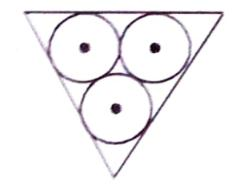
\includegraphics[width=2.5cm]{figs/figure.png}
    \label{fig:figure}
\end{figure}
\begin{enumerate}
\item $4+2\sqrt{3}$
\item $6+4\sqrt{3}$
\item $12+\frac{7\sqrt{3}}{4}$
\item $3+\frac{7\sqrt{3}}{4}$
\end{enumerate}
\hfill (2005S)

\item In a triangle $ABC$, $a, b, c$  are the lengths of its sides and $A, B, C$ are the angles of triangle $ABC$. The correct relation is given by
\begin{enumerate}
\item $\brak{b-c} \sin \brak{\frac{B-C}{2}} = a \cos \brak{\frac{A}{2}}$
\item $\brak{b-c} \cos \brak{\frac{A}{2}} = a \sin \brak{\frac{B-C}{2}}$
\item $\brak{b-c} \sin \brak{\frac{B+C}{2}} = a \cos \brak{\frac{A}{2}}$
\item $\brak{b-c} \cos \brak{\frac{A}{2}} = a \sin \brak{\frac{B+C}{2}}$
\end{enumerate}
\hfill (2005S)

\item One angle of an isosceles $\triangle$ is $120\degree$ and radius of its incircle $= \sqrt{3}$. Then the area of the triangle in sq. units is 
\begin{enumerate}
\item $7+12\sqrt{3}$
\item $12-7\sqrt{3}$
\item $12+7\sqrt{3}$
\item $4\pi$
\end{enumerate}
\hfill (2006 - 3M, -1)

\item Let $ABCD$ be a quadrilateral with area $18$, with side $AB$ parallel to the side $CD$ and $2AB = CD$. Let $AD$ be perpendicular to $AB$ and $CD$. If a circle is drawn inside the quadrilateral $ABCD$ touching all the sides, then the radius is
\begin{enumerate}
\item $3$
\item $2$
\item $\frac{3}{2}$
\item $1$
\end{enumerate}
\hfill (2007 - 3 Marks)

\item If the angles $A, B$ and $C$ of a triangle are in an arithmetic progression and if $\vec{a}, \vec{b}$ and $\vec{c}$ denote the lengths of the sides opposite to $A, B$ and $C$ respectively, then the value of the expression $\frac{a}{c}\sin 2C + \frac{c}{a} \sin 2A$ is
\begin{enumerate}
\item $\frac{1}{2}$
\item $\frac{\sqrt{3}}{2}$
\item $1$
\item $\sqrt{3}$
\end{enumerate}
\hfill (2010)

\item Let $PQR$ be a triangle of area $\Delta$ with $a=2, b= \frac{7}{2}$ and $c=\frac{5}{2}$, where $\vec{a}, \vec{b}$ and $\vec{c}$ are the lengths of the sides of the triangle opposite to the angles at $P, Q$ and $R$ respectively. Then $\frac{2\sin P - \sin 2P}{2\sin P + \sin 2P}$ equals
\begin{enumerate}
\item $\frac{3}{4\Delta}$
\item $\frac{45}{4\Delta}$
\item $\brak{\frac{3}{4\Delta}}^2$
\item $\brak{\frac{45}{4\Delta}}^2$
\end{enumerate}
\hfill (2012)

\item In a triangle the sum of two sides is $\vec{x}$ and the product of the same sides is $\vec{y}$. If $x^2-c^2=y$, where $\vec{c}$ is the third side of the triangle, then the ratio of the inradius to the circum-radius of the triangle is
\begin{enumerate}
\item $\frac{3y}{2\brak{x+c}}$
\item $\frac{3y}{2c\brak{x+c}}$
\item $\frac{3y}{4x\brak{x+c}}$
\item $\frac{3y}{4c\brak{x+c}}$
\end{enumerate}
\hfill (JEE Adv. 2014)

%\end{enumerate}